%Die Angabe des schlauen Spruchs auf diesem Wege funtioniert nur,
%wenn keine Änderung des Kapitels mittels den in preambel/chapterheads.tex
%vorgeschlagenen Möglichkeiten durchgeführt wurde.
\chapter{Machine Learning For Classification}
\label{chap:chapter3}
%\vspace{-3cm}
%\vspace{2cm}
An \emph{algorithm} is a set of instructions used to convert input values to an output, based on certain rules. Consider an example where we need to find all even numbers from a dataset. Here, we can set up a \emph{rule} that if a number is completely divisible by two then it should be included in the output dataset, otherwise not. Naturally, as there can be more than one way to solve a problem, there can be more than one algorithm to solve it. However, there are certain examples where formation of set of rule is practically infeasible. For an example, consider a handwriting recognition software used to scan handwritten forms. Figure~\ref{fig:charrec} illustrates the problem at hand, where a simple character can be written in a number of ways. It is interesting to note that humans are able to read this data without a trouble, but it is really difficult to infer a set of rules which would result in an accurate recognition with help of an algorithm. Machine learning is employed in such cases. Specifically \emph{Machine Learning} (ML) is programming computers to optimize a performance criterion (e.g. character recognition) using example data or a past experience \cite{Alpaydin2004}. 

\begin{figure}[h]
  \begin{center}
    \captionsetup{justification=centering}
    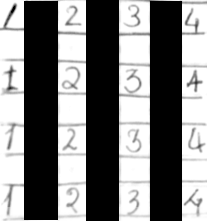
\includegraphics[scale=0.5]{figures/charrec.png}
    \caption{Example of Machine Learning: Character recognition}
    \label{fig:charrec}
  \end{center}
\end{figure}

In case of a handwriting recognition system, an \enquote{example data}, in the form of images of handwritten characters with their \emph{labels}, \emph{i.e.} a number or an alphabet, which each image represents, is collectively referred to as a \emph{training set}, and is used to teach machine learning how a character with the given label would look like, so that ML can recognize when it encounters similar data in the future. Machine learning can be applied in a wide range of applications, where it is not possible to the express human expertise, but a large amount of sample data is available. Typical applications of machine learning include computer vision, pattern recognition, spam filtering, search result optimization etc. 

\section{Types of learning algorithms}
\label{sec:secmltypes}
Based on whether we know labels for the data, ML algorithms can be can be classified in two major categories - supervised learning and unsupervised learning. 

\emph{Supervised learning} algorithms are used when labels of the data to be are known. A spam filter is a good example where supervised learning can be used for \emph{classification}. Here we know an email received is either "spam" or "not-spam", these categories can be used as labels for the sample population and learning algorithm can classify within these two type.  One more application of supervised learning is to predict a numerical value in \emph{regression}. Consider a problem to predict value of a used property, the input parameters in this case are the initial value, year of the construction, size of the property, the locality and so on, whereas the output is the current resale value. one can construct a training set of known resale values and receptive values of input parameters and train the leaning algorithm to predict other inputs. To generalize, aim in supervised learning is to learn mapping from input to output whose correct vales are provided by supervisor \cite{Greene2008}.

\emph{Unsupervised learning} is used in classification problems where the labels for the data are not known. An example of such problem is data clustering \cite{Jain1988}. One of applications of this is to cluster news reports which belong to the same category like sport, science, art and so on. The number and the labels of categories in this case are not defined, and the machine learning application needs to cluster articles based on some common words, and provide the supervisor data, which he may use to label the clustered groups. The aim in supervised learning it to find out regularities or correlation the  input data, without explicit need of a supervisor \cite{Marinai2008}

In case of fault classification, a classification taxonomy has been discussed in earlier chapter. The sample population, which we would generate in our case will contain labels. This makes our case as supervised classification problem. In following subsection, we define the basic terms as applied to case of supervised learning.

\section{Basic terms in supervised machine learning}

A \emph{feature} $(x_i)$ is a result of measurement made on a unit input data. Generally, a set of features $(\boldsymbol{x})$ is needed to characterize a unit of input data and is expressed as,
\[ \boldsymbol{x} = \left[ x_1, x_2, \ldots x_m \right]^T \]  
Its label $l$ denotes the class $C_i \in \{C_1, C_2 \ldots C_k\}$ it belongs to and it is denoted as,
\[ l_i = \left\{ \begin{array}{ll}
         1 & \mbox{if $\boldsymbol{x} \in C_i$};\\
         0 & \mbox{if $\boldsymbol{x} \in C_j, j \neq i$}\end{array} \right. \] 
The \emph{training set} $X$ is then defined as a set containing $N$ values of such examples,
\[ X = \{\boldsymbol{x}^t , \boldsymbol{l}^t \}_{t=1}^N  \]
The aim for machine learning algorithm is to learn data and their labels in the training set and then classify the new examples $\boldsymbol{x}$ by estimating the value of $C(\boldsymbol{x})$. To achieve this, the algorithm tries to find out a hypotheses for every class, $h_i, i \in\{1,2, \ldots k\}$ from a set of all possible hypotheses such that,
\[ h_i(\boldsymbol{x}) = \left\{ \begin{array}{ll}
         1 & \mbox{if $\boldsymbol{x} \in C_i$};\\
         0 & \mbox{$\boldsymbol{x} \in C_j, j \neq i$}\end{array} \right. \] 
The \emph{empirical error} after training is calculated as,
\[ E(\{h\}_{i=1}^k|X) = \sum\limits_{t=1}^N \sum\limits_{i=1}^k | h_i(\boldsymbol{x}) \neq l_i^t ) | \]

Figure~\ref{fig:mlfitting} shows two possible hypotheses $h_1$ , $h_2$ and the actual boundary of classification $C$. For a simple 2-class classification problem, both the hypotheses have the same value of empirical error. If we choose hypothesis $h_1$ then the examples which lie in region between $h_1$ and $C$ will get incorrectly classified and this is called as \emph{overfitting}. On the other hand, if we choose $h_2$ then same will happen for examples in the region between $C$ and $h_2$, called \emph{underfitting}. To check if overfitting or underfitting is has occurred, typically one more labeled dataset called as \emph{cross-validation set} is picked. The empirical error is then calculated over this set and hypotheses obtained during training and the hypothesis with least value of error is then selected. 

\begin{figure}[h]
  \begin{center}
    \captionsetup{justification=centering}
    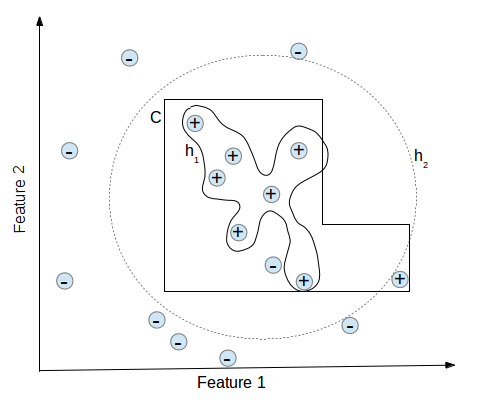
\includegraphics[scale=0.45]{figures/mlfitting.png}
    \caption{Example of overfitting and underfitting}
    \label{fig:mlfitting}
  \end{center}
\end{figure}
In this report, the term \emph{sample population} collectively for the training set and the cross-validation set.

\section{Machine Learning Algorithms for Classification}
\label{sec:c3mlclassification}
This section provides a brief overview of some of the most frequently used machine learning algorithms for the classification problem. It includes advantages and disadvantages for individual algorithms.

\subsection{Naive Bayes}
Naive Bayes is one of the simplest algorithms for learning, more interestingly in some cases it may outperform most of the sophisticated learning algorithms \cite{John1995}. The naive Bayes uses maximum-likelihood estimation to classify new examples. It is based on the Bayes' theorem which states,
\[ P(A|B) = \frac{P(B|A) \times P(A)}{P(B)} \]
Where $P(A)$, $P(B)$ being the probabilities of A and B, and $P(A|B)$ and $P(B|A)$ are conditional probabilities of A, given B and B, given A respectively.
 
During the training of the naive Bayes, the probability of finding an example of each class in the sample population is calculated and stored as the \emph{prior} probability for that class. It also calculates probability for instances $\boldsymbol{x}$ given its class $c$. Under the assumption that attributes in $\boldsymbol{x}$ are independent, it simply becomes a product of probabilities of each single attribute \cite{Williams2006}.
Hence Bayesian theorem, when applied to classification problem using Naive Bayes, becomes
\[ P(C_i|\boldsymbol{x}) = \frac{P(\boldsymbol{x}|C_i) \times P(C)}{P(\boldsymbol{x})}\]
The probability $P(C_i|\boldsymbol{x})$ is referred to as \emph{posterior} probability. A class $C_i$ is chosen if $P(C_i|x) = \max\limits_{k} \{ P(C_k|x)\}$, \emph{i.e.} the class with highest posterior probability.

A clear advantage of using the naive Bayes is that, it is fast to train and fast to classify the data. This is because it needs to scan the database to compute probabilities and store it in a table during training and use this table to classify future examples. Also the naive Bayes is inherently more robust against irrelevant features \cite{Kim2008}, as the likelihood of a class is product of probabilities of each single attribute. On the other hand for prior probabilities to be realistic, the sample population needs to be truly representative of the actual data. Another major disadvantage is that the classifier assumes features to be independent of each other. However in many cases Naive Bayes classifier performs reasonably well even in cases where features are dependent on each other \cite{John1995, Williams2006}.

\subsection{Decision Trees}
\emph{Decision trees} are hierarchical models, wherein each step is a simple threshold-test function of nominal value of a feature against a fixed threshold value \cite{Kotsiantis2013}. The steps in the hierarchy are called as \emph{decision nodes} and a \emph{test} is implemented in the form of a function on features $\boldsymbol{x}$ of an example, with discrete outcomes represented as branches. These nodes apply tests recursively on a feature or a set of features of the  example data, until it flows down the tree and hits a \emph{leaf node}, which represents the output (class in case of classification) \cite{Alpaydin2004}. A simple decision tree is illustrated in figure~\ref{fig:desctree}.

\begin{figure}[h]
  \begin{center}
    \captionsetup{justification=centering}
    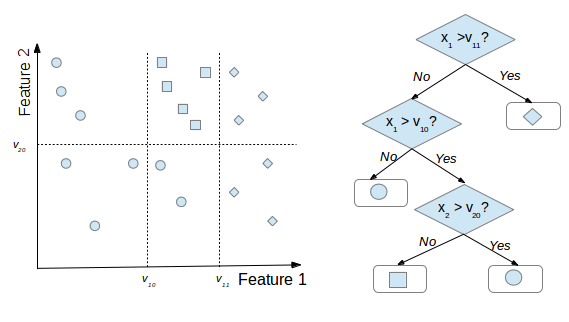
\includegraphics[scale=0.65]{figures/desctree.png}
    \caption{Example of decision tree}
    \label{fig:desctree}
  \end{center}
\end{figure}

In terms of a computer program, this algorithm devices a set of rules which can be interpreted as nested \texttt{IF-ELSE} structure. The \emph{decision tree learning} algorithms are used to derive decision trees. ID3, C4.5 are some examples of these algorithms \cite{Mitchell1997}. ID3 \cite{Quinlan1986} is the simplest of these algorithms. In the case of decision trees, training is to choose features which provides the most information about training set. It then constructs tree using top-down approach. Other advanced algorithms like RIPPER \cite{Cohen1995} build upon the same approach and then employ \emph{pruning} to reduce the training error.

Decision trees use a \enquote{white-box} approach, wherein the internal decision making and structure of tree is visible to user. This also makes decision trees easy to visualize and interpret \cite{Kotsiantis2013}. Decision trees also perform a feature screening to put less informative features near leaf nodes, by its construction.A disadvantage of decision trees is that they can create over-complex trees that do not generalize the data well, \emph{i.e.} the overfitting of data. The problem of learning decision trees is known to be NP-complete hence its worst-case training speed can be slow \cite{Hyafil1976}.

\subsection{Multi-Layer Perceptrons}
\emph{Multi-Layer Perceptrons} (MLP) is a type of artificial neural network models and has been in use since the early 80's. In this model, each feature and output are represented as nodes, and feature nodes in each layer are connected to the upper layer using weights or \emph{synapses}. Figure~\ref{fig:perceptron} is an example of a simple, two layered perceptron. Inputs $x_1, x_2 \ldots x_k$ are features and $x_0 = +1$ is a \emph{bias element}, used to make model more general by allowing user to fine-tune the the output by shifting the output function. $\boldsymbol{a,b}$ are matrices of weights on the synapses in the first to the hidden layer and the hidden layer to the output, respectively.

\begin{figure}[h]
  \begin{center}
    \captionsetup{justification=centering}
    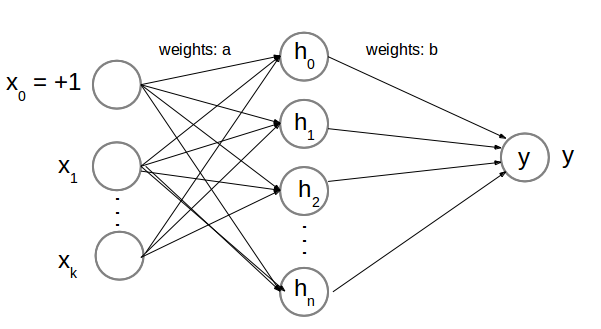
\includegraphics[scale=0.45]{figures/perceptron.png}
    \caption{Two layered perceptron}
    \label{fig:perceptron}
  \end{center}
\end{figure}

The output of perceptron in figure~\ref{fig:perceptron} can be represented mathematically as
\[ y = \sum\limits_{j=0}^n b_j (\sum\limits_{i=1}^k (a_{ij}x_i + a_0))\]
During the training of a perceptron, the training algorithm will try to find the appropriate connecting weights. Multiple layers of perceptrons can be constructed by implementing a hidden layer of nodes between features and output, by doing so one can implement non-linear output functions. The degree of non-linearity depends on the number of hidden layers. Back-propagation algorithm \cite{Rumelhart1985} is one of commonly used algorithm for training MLPs. It works by calculating error correlations at each output and use these to calculate the error terms in previous layers and so on. The error terms are then used to adjust weights of the individual synapses. 

The error function in this case is defined as,

\[ E(\boldsymbol{a},\boldsymbol{b}|X) = \frac{1}{2} \sum\limits_{t} (l^t - y^t)^2\]

The gradient of this error function is calculated during back-propagation, and weights are updated once the gradient function reaches a local minimum.

Once trained, MLPs are able to classify data fast. They can implement higher order polynomial functions and are flexible and powerful due to well researched mathematical background and variety of training algorithms available, which can be selected according to the application and the amount of data available. A disadvantage is that the network needs to be completely re-trained when new training data is to be added. Selection of features also has a profound impact on the performance of MLPs \cite{Kavzoglu2002, El-Khatib2010}.

\subsection{Support Vector Machines}
\label{mltypes:svm}
\emph{Support Vector Machines} (SVMs) have existed for a long time, but the research on these gained particular momentum since Vapnik \cite{Vapnik1995} evaluated these methods in his book on statistical learning theory. SVM belongs to the class of linear classifiers. In higher dimensions, SVM tries to divide the feature space using decision hyperplanes. However, as there can be several planes that divide feature space, SVM selects the plane with maximum distance from support vectors. Figure~\ref{fig:svm1} shows a case where two possible lines divide feature space, $h_1$ and $h_2$. SVM will choose $h_2$ as the \emph{decision boundary} or the \emph{discriminant function} as it provides maximum margin for the classification. The examples with least distance from the decision hyperplane are called \emph{support vectors}.

\begin{figure}[h]
  \begin{center}
    \captionsetup{justification=centering}
    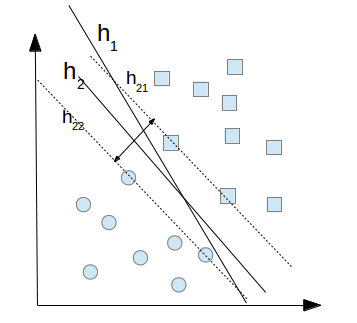
\includegraphics[scale=0.45]{figures/svm1.png}
    \caption{SVM with linear decision boundary}
    \label{fig:svm1}
  \end{center}
\end{figure}
The linear discriminant function used in this case can be expressed as,
\[g(x) = \boldsymbol{w^T}\boldsymbol{x} + w_0 \]
Where $w_0$ denotes a bias, and the vector $\boldsymbol{w}$, called weight vector, is the distance of respective hyperplanes passing through support vectors from the origin.

Referring to figure~\ref{fig:svm1}, hyperplane $h_2$ is actually a result of two hyperplanes, defined by the respective support vectors of two classes. Let $h_{21}$ and $h_{22}$ represent these hyperplanes	such that:
\[\begin{array}{ll} 
h_{21}: \boldsymbol{w^T}\boldsymbol{x} + b = 1 & \mbox{when label is +1};\\
h_{22}: \boldsymbol{w^T}\boldsymbol{x} + b = -1 & \mbox{when label is -1}
\end{array} \]

However as illustrated in the figure~\ref{fig:svm2} the feature space may not be linearly separable at all. In these cases SVM uses \emph{kernel trick} to achieve linearly separable kernel space. The idea behind kernel trick is to apply a function $\phi$ to transform all points in the feature space to a higher dimension, so that resulting feature space is linearly separable. After transformation, the regular SVM algorithm is used for classification.

\begin{figure}[h]
  \begin{center}
    \captionsetup{justification=centering}
    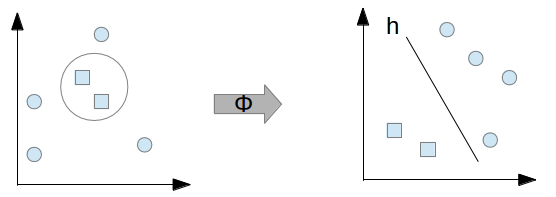
\includegraphics[scale=0.50]{figures/svm2.png}
    \caption{Kernel trick for SVM}
    \label{fig:svm2}
  \end{center}
\end{figure}

This makes the linear discriminant used of the form,
\[\boldsymbol{y} = \boldsymbol{w^T}\phi(\boldsymbol{x}) + w_0 \]

where $\phi$ denotes the function used to convert the non-linear feature space to linear one.

Let $||\boldsymbol{w}||$ denote the distance between these hyperplanes, C a constant to adjust variance and to minimize the training error $\xi$ . Then the training of SVM is to find a maximum margin hyperplane, which can be viewed as an optimization problem \cite{Vapnik1995, Chang2011},
\[\begin{array}{ll} 
 \min &\frac{1}{2} ||\boldsymbol{w}||^2 + C \sum\limits_{i=1}^n \xi_i \\
 \mbox{subject to} & l^t(\boldsymbol{w^T}\phi(\boldsymbol{x}) + w_0) 
\end{array}\]

This QP may be difficult to solve as function $\phi(\boldsymbol{x})$ can be high in dimensions. Making the mapping used computationally expensive \cite{Ben-Hur2010}.

To solve this, suppose $\boldsymbol{w}$ can be expressed as $\boldsymbol{w} = \sum\limits_{i=1}^n \alpha_i\boldsymbol{x_i}$ (dual of this problem), and also define a \emph{kernel function},
\[K(\boldsymbol{x},\boldsymbol{x_i}) = \phi(\boldsymbol{x})\phi^T(\boldsymbol{x_i})\]
 Substituting this in minimization problem reduces the dimensionality back to the original.

Most commonly used kernels are:
\begin{description}
  \item[Linear] $K(\boldsymbol{x},\boldsymbol{x_i}) = \boldsymbol{x}^T\boldsymbol{x_i}$
  \item[Polynomial] $K(\boldsymbol{x},\boldsymbol{x_i}) = \gamma(\boldsymbol{x}^T\boldsymbol{x_i}+r)^d, \gamma > 0$
  \item[Radial Basis Function (RBF)] $K(\boldsymbol{x},\boldsymbol{x_i}) = \mathrm{e}^{-\gamma||\boldsymbol{x}-\boldsymbol{x_i}+r)||^2}, \gamma > 0$
  \item[Sigmoid] $K(\boldsymbol{x},\boldsymbol{x_i}) = \tanh(\gamma\boldsymbol{x}^T\boldsymbol{x_i}+r)$
\end{description}

$\gamma$, $r$ and $d$ are the kernel parameters.

The advantage of using SVM is its ability to tackle non-linear data. By using a variety of kernels like linear, polynomial, RBF and so on, the user has flexibility to classify the data with non-linear feature spaces \cite {Chang2011}. Handling higher dimensional features spaces is also not an issue, because of the theoretical framework \cite{Vapnik1995} supports an $n$-dimensional space. SVMs also provide a unique solution as the optimality problem is convex, which is an advantage as compared to neural networks, which can provide solutions at a local minimum \cite{Auria2008}. SVM, being a maximum margin classifier, avoids underfitting of data. One the other hand, training an SVM is solving an quadratic optimality problem (known to be NP hard), hence it can take a long time to train when datasets are large. Also, a common disadvantage of SVM is that the model it constructs is a \enquote{black-box} approach to classify the data, specially when the feature set is large \cite{Auria2008}.

